\documentclass[11pt]{article}
\usepackage[margin=1in]{geometry}
\usepackage[T1]{fontenc}
\usepackage{lmodern}
\usepackage{microtype}
\usepackage{booktabs}
\usepackage{amsmath,amssymb}
\usepackage{graphicx}
\usepackage{hyperref}
\usepackage[numbers,sort&compress]{natbib}
\usepackage{caption}
\captionsetup{font=small}

\title{Cross-Dataset Flow-Based Intrusion Detection: A Seven-Dataset Benchmark and Negative Results for Label-Free Transfer}
\author{Quang-Vinh Dang\\
British University Vietnam, Hung Yen, Vietnam\\
\texttt{vinh.dq4@buv.edu.vn}\quad ORCID 0000-0002-3877-8024}
\date{}

\begin{document}
\maketitle

\begin{abstract}
Machine-learning detectors of malicious network flows reach 0.985 ROC-AUC when trained and tested on the same dataset and then lose most of that skill on another network.
We build a benchmark of eight public flow datasets from five laboratories and three flow extractors, harmonised to features of the same physical meaning, and evaluate seventeen methods and variants in 42 ordered source--target transfers and seven leave-one-dataset-out (LODO) tasks over three seeds.
Classical tree ensembles score 0.54 to 0.56 ROC-AUC on average across transfers, 36 to 48\% of the transfers are below chance, and even transfer between two datasets from the same laboratory is below chance (0.44 for CatBoost).
We designed a domain-invariant method, RIFT, with per-domain rank normalisation anchored on benign traffic, invariance-driven feature selection and test-time label-shift correction.
It does not work: it is below its own gradient-boosting baseline (0.484 against 0.557 pairwise ROC-AUC, 0.519 against 0.630 LODO), and every ablation points to the transductive components, in particular its estimate of the target attack prior, which has a mean absolute error of 0.41.
CORAL and DANN do not improve on plain gradient boosting either.
Controls rule out the most obvious implementation explanations: the same pipeline reaches 0.985 in-domain, no common flow feature keeps the sign of its association with the attack label across the datasets (0 of 14), a classifier recognises the source dataset of a flow with 91.5\% accuracy, and nearest-neighbour agreement in the region where datasets overlap is near chance (median Cohen's $\kappa$ 0.03 over 19 pairs).
Source pre-training does not help the few-label setting on average: fine-tuning a source-trained model on 0.1\% of the target labels reaches 0.835 ROC-AUC, below the 0.928 of a model trained on those labels alone.
We conclude that these datasets disagree on the labelling function of flows and not only on feature scales, and that methods that assume a fixed $P(y\mid x)$ should not be expected to repair it.
The package, configurations and all raw results are public.
\end{abstract}

\section{Introduction}
Flow-based network intrusion detection is usually evaluated by splitting one dataset into a training and a test part.
Under that protocol gradient-boosted trees exceed 0.99 ROC-AUC on CIC-IDS2017 and USB-IDS-1.
A growing literature shows that the same models degrade sharply on a second dataset \citep{layeghy2023explainable,cantone2024crossdataset,dhooge2020inter,dhooge2023damaged,apruzzese2022cross}, and even datasets from one laboratory transfer poorly.
Two explanations are common.
The first is covariate shift: capture tools, link speeds and traffic mixes change the scale and distribution of features, which normalisation or domain adaptation could repair \citep{ganin2016dann,sun2016coral,layeghy2023dinids}.
The second is that the datasets define attacks differently, so that the same flow statistics carry different labels, which no unlabelled adaptation can repair.

This paper separates the two as far as a benchmark allows, and it reports a negative result in full.
We make four contributions.
\begin{enumerate}
\item \textbf{A benchmark} of seven public datasets (an eighth, CTU-13, supports only a minimal feature tier; Table~\ref{tab:datasets}) with a common flow schema, a bottom-$k$ hash sampler that gives a reproducible uniform sample of distinct rows, and a protocol with in-domain, pairwise (42 ordered pairs, labelled by whether the pair shares a laboratory or an extractor) and LODO settings, in inductive and transductive modes, over three seeds.
\item \textbf{A method designed to work, and its failure.} RIFT combines per-domain rank normalisation anchored on benign traffic, invariance-driven feature selection, and test-time label-shift correction. We evaluate it with a full ablation and show that it is below its own baseline.
\item \textbf{Controls} that answer the objection that a negative result may be an implementation failure: positive controls, an oracle search over model family, normalisation and feature subsets, a nearest-neighbour test of whether the same flow statistics carry the same labels across datasets, a dataset-identity classifier, and a fair few-label comparison.
\item \textbf{An honest account of what the controls do and do not show}, including that the oracle search covers only two pairs and that the concept-shift evidence is correlational.
\end{enumerate}
A companion study builds a few-label meta-learner on the diagnosis made here; this paper is self-contained.

\section{Related work}
\citet{layeghy2023explainable} train on one NetFlow-v2 dataset and test on another and report attack-class F1 below 1\% for several pairs of CIC-IDS2018, UNSW-NB15 and ToN-IoT, with strongly asymmetric results; a domain-invariance method of the same group \citep{layeghy2023dinids} improves some pairs.
\citet{cantone2024crossdataset} report MCC between 0.26 and 0.44 when CIC-IDS2017 and CIC-IDS2018 are exchanged, even though both come from the same laboratory.
\citet{dhooge2020inter,dhooge2023damaged} analyse inter-dataset generalisation per attack class and the effect of data-damaged models on it.
\citet{catillo2022transferability} study transfer from CIC-IDS2017 to USB-IDS-1 \citep{catillo2021usbids1}, which share an extractor, and \citet{apruzzese2022cross} cross-evaluate per-attack detectors across several networks.
\citet{engelen2021troubleshooting} document labelling errors in CIC-IDS2017, and \citet{arp2022dos,apruzzese2023sok} discuss pitfalls of machine-learning evaluation in security.
\citet{sarhan2022standard} propose standard NetFlow feature sets to ease cross-dataset use.
Our benchmark differs in covering seven datasets and three extractors with one schema, in labelling each pair by how much infrastructure the two datasets share, in running label-free transfer methods against default-setting baselines over three seeds, and in reporting the controls that decide whether the negative result is a finding.
On the method side, we compare against domain-adversarial training \citep{ganin2016dann} and correlation alignment \citep{sun2016coral}, and RIFT uses the expectation-maximisation correction of the output prior of \citet{saerens2002adjusting}.

\section{Benchmark}
\paragraph{Datasets.}
Table~\ref{tab:datasets} lists the datasets: CIC-IDS2017 \citep{sharafaldin2018cicids} and CIC-IDS2018, USB-IDS-1 \citep{catillo2021usbids1}, InSDN \citep{elsayed2020insdn}, UNSW-NB15 \citep{moustafa2015unsw}, ToN-IoT \citep{alsaedi2020toniot}, IoT-23 \citep{garcia2020iot23} and CTU-13 \citep{garcia2014ctu13}.
They come from five laboratories (UNB, Sannio, UCD, UNSW Canberra and the Stratosphere laboratory of CTU) and three extractors (CICFlowMeter, Argus and Zeek).
CIC-IDS2017 and CIC-IDS2018 share a laboratory and an extractor, UNSW-NB15 and ToN-IoT share a laboratory, and IoT-23 and CTU-13 share a laboratory.
The attack prior of the distinct rows ranges from 0.15 (CIC-IDS2017, CIC-IDS2018) to 0.93 (USB-IDS-1).
Labels are binary, because attack taxonomies differ across datasets; the raw attack type is kept for per-family analysis.
CTU-13 supports only a minimal feature tier and is therefore used only in the companion study, so the benchmark proper has seven datasets and 42 ordered pairs.

\begin{table}[t]
\centering\small
\caption{Datasets. The attack prior is that of the distinct rows after harmonisation. CTU-13 supports only the minimal feature tier and is excluded from the seven-dataset benchmark.}\label{tab:datasets}
\begin{tabular}{lllcc}
\toprule
Dataset & Laboratory & Extractor & Attack prior & Feature tier \\
\midrule
CIC-IDS2017 & UNB CIC & CICFlowMeter & 0.152 & core \\
CIC-IDS2018 & UNB CIC & CICFlowMeter & 0.149 & core \\
USB-IDS-1 & Univ. of Sannio & CICFlowMeter & 0.930 & core \\
InSDN & UCD & CICFlowMeter & 0.640 & core \\
UNSW-NB15 & UNSW Canberra & Argus, Bro & 0.464 & core \\
ToN-IoT & UNSW Canberra & Zeek & 0.743 & core \\
IoT-23 & Stratosphere, CTU & Zeek & 0.486 & core \\
CTU-13 & Stratosphere, CTU & Argus & 0.570 & minimal \\
\bottomrule
\end{tabular}

\end{table}

\paragraph{Common flow schema.}
Extractors export different features, so only features with the same physical meaning and units are used.
The core tier has five base features (duration, forward and backward packets, forward and backward bytes) and eight derived rates and ratios (13 features), all computed after harmonisation and passed through $\log(1+x)$.
Ports and protocol are excluded because two of the datasets do not export them.
Window-size and inter-arrival features exist only for some extractors and are excluded from the core tier.
Alias tables resolve the different spellings of CICFlowMeter columns, repeated header rows of CIC-IDS2018 are removed, and negative sentinel values are clipped to zero.

\paragraph{Sampling.}
Each cleaned row receives a seeded 64-bit hash of all harmonised features the dataset provides (rounded to $10^{-6}$) and its label, so distinctness is with respect to the full feature set of the dataset.
Per label we keep the 100\,000-row budget of rows with the smallest hash (a bottom-$k$ sketch), so that duplicated flows occupy one slot and the sample is uniform over \emph{distinct} rows.
The attack prior is defined on distinct rows, and a class that is short shrinks the sample instead of being back-filled.
This makes the benchmark a distinct-row benchmark, so absolute numbers are not comparable with studies that keep duplicates.

\paragraph{Protocol.}
Each dataset is split 70/30, stratified and seeded.
Sources train on their training split and the target is evaluated on its test split.
In the transductive mode a method also sees the unlabelled features of the target training split, disjoint from the evaluated rows; in the inductive mode it sees nothing from the target.
The in-domain setting is the upper reference.
The pairwise setting uses all 42 ordered pairs of the seven core datasets, each labelled \emph{same family} (same laboratory, 4 pairs), \emph{same extractor} (different laboratory, 12 pairs) or \emph{cross-extractor} (26 pairs).
In LODO a method trains on the other six datasets pooled.
Target labels are never used for training, model selection or threshold tuning; threshold-dependent metrics use the decision rule of the method.
The sample is drawn once; seeds 0, 1 and 2 change the 70/30 split and the model randomness, and we average seeds within a scenario before computing statistics over scenarios.
Metrics are ROC-AUC (headline), PR-AUC, F1, balanced accuracy, MCC, recall and false-positive rate.

\paragraph{Methods.}
Baselines use a global standard scaler fitted on the sources: logistic regression, random forest (300 trees), histogram gradient boosting (HGB), CatBoost \citep{prokhorenkova2018catboost} with 500 iterations, XGBoost, and a two-layer MLP.
We add CORAL \citep{sun2016coral} followed by HGB, and DANN \citep{ganin2016dann}; both are transductive.
RIFT is described next.

\section{RIFT: a method designed to work}
RIFT targets three sources of failure separately.
\emph{Covariate shift} is addressed by domain-wise normalisation: each domain is mapped to Gaussian ranks computed on its own features.
On source domains the normaliser is fitted on benign rows only, because benign traffic is the stable background of a network.
On the target, where labels are unknown, the anchor set is the $\gamma=0.8$ fraction of the $(1-\hat\pi_t)$ lowest-scoring rows under the current estimate $\hat\pi_t$ of the target attack prior, and the target is transported into the source representation by quantile matching against an equally truncated reference of source benign rows.
\emph{Spurious dataset-specific cues} are addressed by invariance-driven feature selection: a feature is kept only if the sign of its univariate association with the label is identical in every source and its minimum strength is at least 0.05; with a single source and a target pool (transductive mode), the 25\% of features with the largest Kolmogorov--Smirnov distance between source and target are dropped, and without a target pool all features are kept; at least six features are always retained.
\emph{Label shift} is addressed by the expectation-maximisation correction of the output prior of \citet{saerens2002adjusting}, applied after isotonic calibration.
The classifier is HGB.
Ablations remove one component at a time (domain normalisation, anchor, selection, prior correction), replace the rank transform by robust or z-score scaling, start the anchor from the pooled rather than the source normaliser, and add uncertainty-gated self-training.

\section{Results}
\subsection{In-domain skill does not transfer}
Table~\ref{tab:main} gives ROC-AUC by setting.
In-domain, the boosted ensembles reach 0.985 (random forest 0.981) averaged over the seven datasets (CatBoost between 0.950 on IoT-23 and 1.000 on ToN-IoT and USB-IDS-1), logistic regression 0.923.
Across the 42 pairs the tree ensembles reach 0.54 to 0.56 (CatBoost 0.559, HGB 0.557, XGBoost 0.550, random forest 0.538) and DANN 0.565.
Between 36\% (HGB) and 48\% (random forest) of the pairs are below 0.5 for the tree ensembles (21 to 29\% are below 0.40), so on those pairs the learned rule ranks attacks as \emph{less} suspicious than benign flows on the target.
Only 3 of 42 pairs reach 0.9 for CatBoost, and all three involve USB-IDS-1 (USB-IDS-1$\rightarrow$ToN-IoT 0.920, ToN-IoT$\rightarrow$USB-IDS-1 0.948, InSDN$\rightarrow$USB-IDS-1 0.959); the extreme pair is CIC-IDS2018$\rightarrow$CIC-IDS2017 at 0.232.
Pairs from the same laboratory, which are the easiest on paper, are on average the worst and are strongly asymmetric: CatBoost scores 0.44 on the four same-family pairs (CIC-IDS2017$\rightarrow$CIC-IDS2018 0.75 but the reverse 0.23, ToN-IoT$\rightarrow$UNSW-NB15 0.44, UNSW-NB15$\rightarrow$ToN-IoT 0.34), 0.64 on same-extractor pairs and 0.54 on cross-extractor pairs; with four pairs and one favourable direction we do not test this ordering.
LODO is better because six sources are pooled, but still 0.65 for CatBoost, and it varies from 0.968 on USB-IDS-1 to 0.333 on IoT-23 (Table~\ref{tab:targets}).

\begin{table}[t]
\centering\small
\caption{ROC-AUC, mean over scenarios (seeds averaged within a scenario). Pairwise columns split the 42 ordered pairs by what the two datasets share. LODO: train on the other six datasets pooled. Transductive mode; the non-adaptive methods are unaffected by the mode up to run-to-run noise (at most 0.003).}\label{tab:main}
\begin{tabular}{lrrrrr}
\toprule
Method & In-domain & Same family & Same extractor & Cross-extractor & LODO \\
 & (7) & (4 pairs) & (12 pairs) & (26 pairs) & (7) \\
\midrule
LR & 0.923 & 0.341 & 0.472 & 0.503 & 0.480 \\
RF & 0.981 & 0.478 & 0.597 & 0.521 & 0.574 \\
HGB & 0.985 & 0.480 & 0.643 & 0.529 & 0.630 \\
CatBoost & 0.985 & 0.440 & 0.637 & 0.541 & 0.652 \\
XGBoost & 0.985 & 0.397 & 0.642 & 0.532 & 0.612 \\
MLP & 0.981 & 0.453 & 0.621 & 0.539 & 0.503 \\
CORAL & 0.985 & 0.494 & 0.494 & 0.542 & 0.631 \\
DANN & 0.980 & 0.516 & 0.678 & 0.521 & 0.613 \\
RIFT & 0.985 & 0.501 & 0.465 & 0.491 & 0.519 \\
RIFT + self-training & 0.985 & 0.519 & 0.448 & 0.486 & 0.500 \\
\bottomrule
\end{tabular}

\end{table}

\begin{table}[t]
\centering\small
\caption{In-domain and leave-one-dataset-out ROC-AUC per target (inductive).}\label{tab:targets}
\begin{tabular}{lrrr}
\toprule
Target & In-domain & LODO CatBoost & LODO HGB \\
\midrule
CIC-IDS2017 & 0.999 & 0.803 & 0.775 \\
CIC-IDS2018 & 0.970 & 0.656 & 0.684 \\
InSDN & 0.998 & 0.672 & 0.657 \\
IoT-23 & 0.950 & 0.333 & 0.308 \\
ToN-IoT & 1.000 & 0.667 & 0.560 \\
UNSW-NB15 & 0.978 & 0.468 & 0.467 \\
USB-IDS-1 & 1.000 & 0.968 & 0.957 \\
\bottomrule
\end{tabular}

\end{table}

\begin{figure}[t]
\centering
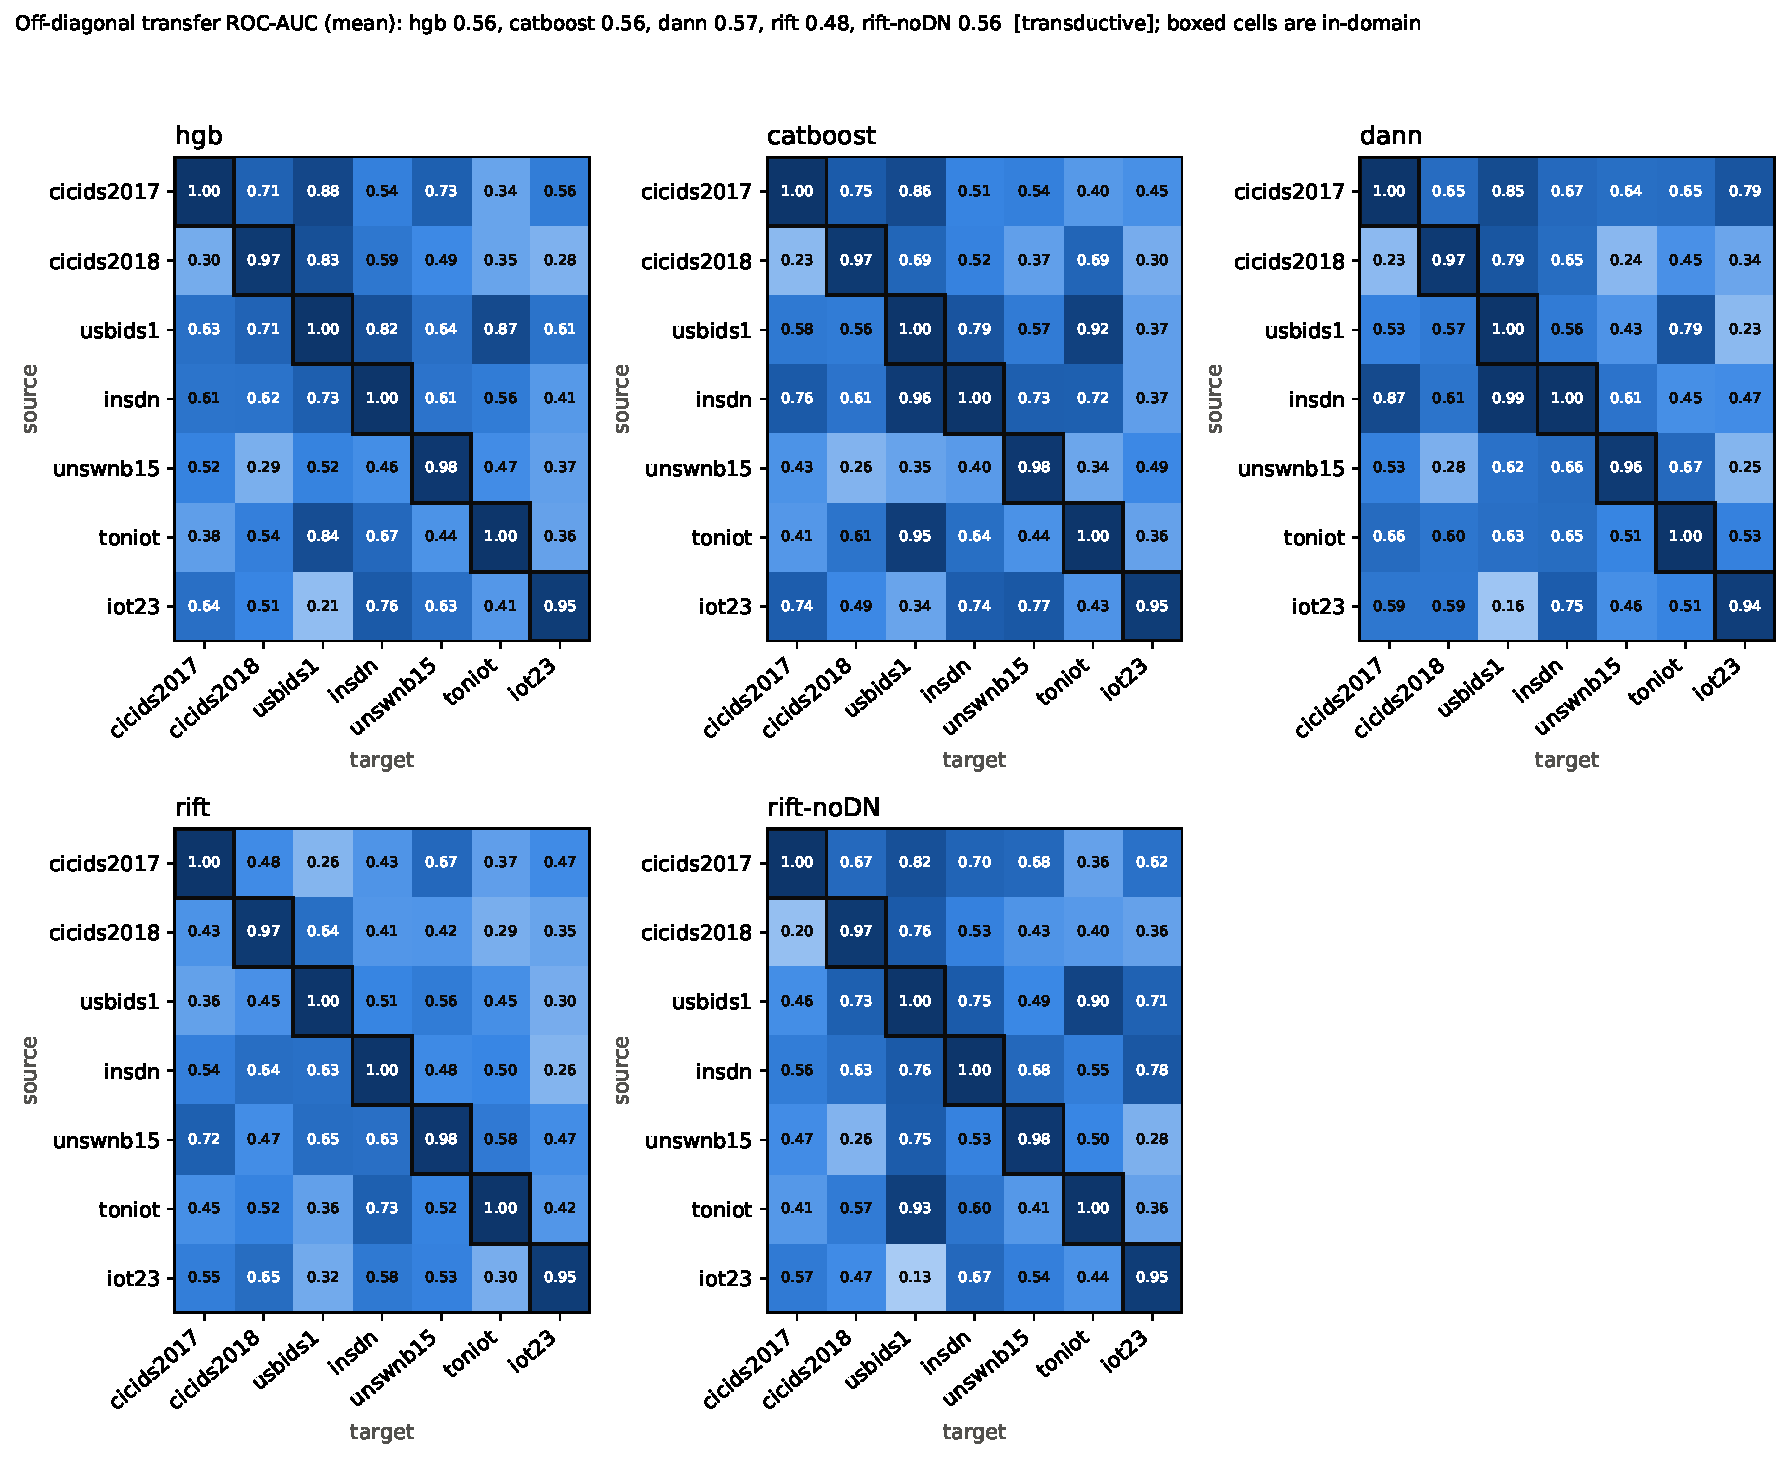
\includegraphics[width=0.9\textwidth]{figures/pairwise_matrix.pdf}
\caption{Source$\rightarrow$target ROC-AUC of the benchmark methods (transductive mode); the boxed diagonal is the in-domain value.}\label{fig:matrix}
\end{figure}

No method is consistently best.
A Friedman test over the 42 pairs finds a difference among the 17 transductive variants ($p=0.006$), but that is driven by the weak methods (logistic regression and the RIFT variants); among the inductive methods ($p=0.74$) and in LODO ($p=0.065$ transductive, $0.47$ inductive) it finds none.
The pairwise differences among CatBoost, HGB, XGBoost and DANN are of the order of 0.01 (in LODO up to 0.04, with CatBoost best on mean rank), far below the spread between pairs; with 7 LODO targets and pairs that share sources and targets, the Friedman tests have little power, so the data neither show nor exclude a best method.
On average CORAL and DANN do not repair transfer: pairwise they are at 0.524 and 0.565, in LODO at 0.631 and 0.613, against 0.630 for HGB, although both differ strongly by target (on LODO IoT-23 CORAL reaches 0.72 and DANN 0.76 against 0.31 for HGB).

\subsection{RIFT fails}
Table~\ref{tab:rift} shows RIFT and its ablations.
RIFT is below its own HGB baseline in both settings (pairwise 0.484 against 0.557, LODO 0.519 against 0.630).
Removing domain normalisation recovers the baseline (0.558 pairwise, 0.620 LODO), and removing the benign anchor recovers part of it (0.538, 0.543), so the target-side normalisation and the benign anchor are what hurt.
Removing the label-shift correction changes nothing (0.484 against 0.484 pairwise), as it must for ROC-AUC, because a prior-ratio adjustment is a monotone transform of the posterior.
In LODO the invariant selection has no effect either, for a mechanical reason: no feature has the same sign in all six sources (consistent with Sect.~\ref{sec:controls}), so the selection falls back to keeping all 13 features in every LODO scenario; in the pairwise setting the Kolmogorov--Smirnov rule keeps 10 of 13.
Replacing the rank transform by robust or z-score scaling does not help (0.479 and 0.485 pairwise).
Self-training does not help (0.478).
In the inductive pairwise setting there is no target pool and a single source, so RIFT keeps all features and reduces to HGB on a monotone rank transform; all variants score the same (0.551 against 0.554 for HGB).
In inductive LODO the per-domain source normalisation and the multi-source selection remain active and the variants differ (RIFT 0.586, without domain normalisation 0.620, robust scaling 0.502); RIFT is below HGB there too (0.630), and removing domain normalisation raises the score without any target data.

\begin{table}[t]
\centering\small
\caption{RIFT and its ablations, transductive mode. Pairwise: 42 pairs; LODO: 7 targets. Prior error (pairwise only): mean absolute error of the estimated target attack prior.}\label{tab:rift}
\begin{tabular}{lrrrr}
\toprule
Method & Pairwise AUC & Pairwise bal. acc. & LODO AUC & Prior error \\
\midrule
HGB & 0.557 & 0.533 & 0.630 & -- \\
RIFT & 0.484 & 0.510 & 0.519 & 0.413 \\
RIFT $-$ domain norm. & 0.558 & 0.536 & 0.620 & 0.385 \\
RIFT $-$ benign anchor & 0.538 & 0.521 & 0.543 & 0.381 \\
RIFT $-$ invariant selection & 0.483 & 0.495 & 0.519 & 0.429 \\
RIFT $-$ prior correction & 0.484 & 0.509 & 0.519 & -- \\
RIFT, pooled init. & 0.487 & 0.500 & 0.498 & 0.421 \\
RIFT, robust scaling & 0.479 & 0.504 & 0.487 & 0.425 \\
RIFT, z-score scaling & 0.485 & 0.498 & 0.510 & 0.414 \\
RIFT + self-training & 0.478 & 0.507 & 0.500 & 0.409 \\
\bottomrule
\end{tabular}

\end{table}

The target-prior estimate is poor, although removing the correction does not matter for ROC-AUC and the prior error is similar for the variants that recover the baseline (0.39 and 0.38 for the variants without domain normalisation and without anchor against 0.41 for RIFT), so the error alone does not explain the loss.
Across the 42 pairs RIFT estimates the target attack prior with a mean absolute error of 0.41 (bias $-0.35$, Pearson correlation with the true prior 0.05); in LODO it estimates an average prior of 0.003 where the true average is 0.51.
The anchor is meant to be benign traffic, but its purity (the fraction of truly benign rows, logged as a diagnostic and never used by the method) is 0.50 in pairwise and 0.47 in LODO transfer, so the anchor is as contaminated with attacks as the pool.
Estimating the prior with a normaliser fitted on the pool (``pooled init.'') does not help (0.487).
We hypothesise, without having tested it, that a source classifier that is inverted on the target gives the EM nothing to correct.

\begin{figure}[t]
\centering
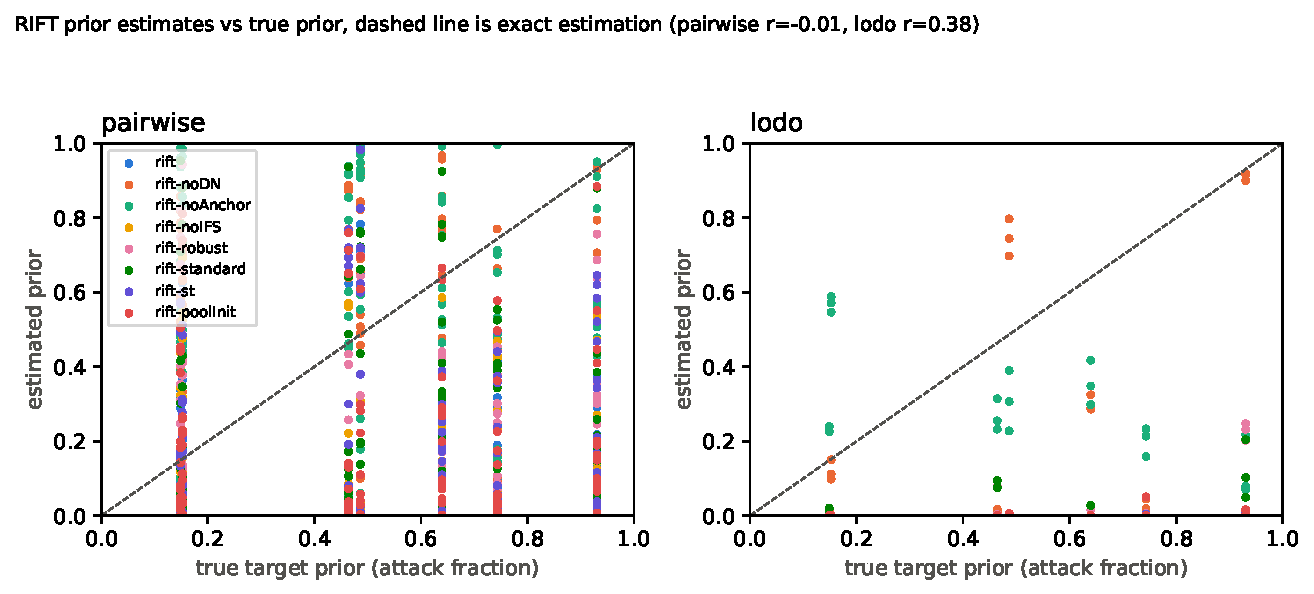
\includegraphics[width=0.75\textwidth]{figures/prior_estimation.pdf}
\caption{Estimated against true target attack prior for the RIFT variants.}\label{fig:prior}
\end{figure}

\subsection{Source data do not help in the few-label setting}
As a reference outside the label-free benchmark, we continue a source-pretrained CatBoost on a labelled budget of 0.1\%, 1\% and 5\% of the target training split (on average 62, 617 and 3\,083 rows), and compare it with CatBoost trained on those rows alone.
At 0.1\%, the source-pretrained model reaches 0.835 and the target-only model 0.928 (Table~\ref{tab:fewshot}).
Giving the continued model 300 or 500 extra trees narrows the gap to 0.911 and 0.914 against 0.932, so the effect is not only a capacity artefact, but it does not reverse: at 1\% and 5\% the two are within 0.001 to 0.002 once the trees are matched.
Source pre-training thus gives no average benefit over target labels for this model family, and a harm at the smallest budget (0.09 AUC with 100 trees, 0.02 with 500); continuing a boosted model by adding trees is a weak way to use source data, and stronger few-label baselines (pooled training with target weighting, source scores as a feature, an in-context model given the source rows) are not part of this study.

\begin{table}[t]
\centering\small
\caption{Few-label comparison over the 42 pairs, ROC-AUC. The continued model starts from a CatBoost trained on the source and adds the stated number of trees on the labelled target rows; the other model uses only those rows.}\label{tab:fewshot}
\begin{tabular}{lrrrr}
\toprule
Setting & Extra trees & 0.1\% labels & 1\% labels & 5\% labels \\
\midrule
Source-pretrained, continued & 100 & 0.835 & 0.950 & 0.966 \\
 & 300 & 0.911 & 0.966 & 0.978 \\
 & 500 & 0.914 & 0.966 & 0.978 \\
Target labels only & 100 & 0.928 & 0.964 & 0.977 \\
 & 300 & 0.932 & 0.967 & 0.980 \\
 & 500 & 0.932 & 0.967 & 0.979 \\
\bottomrule
\end{tabular}

\end{table}

\subsection{Shift and family explanations}
An unsupervised shift score (an isolation forest fitted on the source and applied to the target pool) does not predict transfer skill: the Spearman correlation with zero-shot ROC-AUC over 2\,142 (scenario, method, seed) points is $-0.055$ (nominal $p=0.01$, but the points are not independent; per method $|\rho|\le0.27$ with mixed signs).
Sharing attack types does not obviously predict it either: for every family we compared the informedness of a method on a target family when the source contains that family and when it does not.
Pooled over families (transductive mode), the paired difference for CatBoost is $+0.012$ (95\% half-width 0.088, $p=0.82$) and for HGB $-0.046$ ($p=0.14$); none of the 248 (method, mode, family) tests has $p<0.05$, but each test uses only 3 to 6 paired cells and cannot reach 0.05 with fewer than 6, so the benchmark has too little power to show whether missing attack types matter.

\section{Controls}
A negative result is a finding only if competing explanations are ruled out.
\paragraph{The pipeline works.}
The same pipeline reaches 0.985 in-domain, and a target-only CatBoost with 0.1\% of target labels reaches 0.93, so the features carry the signal and the code can learn it.

\paragraph{Tuning as an explanation (one informative pair).}
For CIC-IDS2017$\rightarrow$CIC-IDS2018 we searched all five model families (HGB, CatBoost, XGBoost, random forest, logistic regression) with two settings of the main hyperparameters, three normalisations (none, global, per-domain rank) and the full feature set or the set without one feature group (264 configurations, seed 0, 30\,000 source rows), and selected the best on the target test split, an optimistic oracle.
It reaches 0.799 against 0.683 for the benchmark HGB, still far from the in-domain 0.97 to 1.00.
For CIC-IDS2017$\rightarrow$USB-IDS-1 only 33 HGB configurations were run and the oracle (0.862) is below the full-data benchmark HGB (0.972), so that pair says nothing about tuning.
The grid is reduced and the source is subsampled, so the result is not an upper bound over all configurations.

\paragraph{The same statistics do not carry the same labels.}
We standardise source and target with source statistics, find for each target row its 10 nearest source rows, and restrict to the \emph{overlap region} (rows whose mean neighbour distance is at most the 90th percentile of source-to-source distances).
There the majority label of the neighbours should agree with the true target label if $P(y\mid x)$ were shared.
Over the 19 pairs with at least 100 overlapping rows (seed 0; 23 of the 42 pairs have fewer) the median Cohen's $\kappa$ is 0.03, 84\% of the pairs have $\kappa\le0.1$ and the maximum is 0.25 (Fig.~\ref{fig:kappa}); three of the 19 values are exactly 0, which a single-class overlap region also produces, and only five are negative, so the pattern is closer to independence than to inversion. The in-domain reference, source-test rows against the same source-train index, has $\kappa$ of 0.91 on average and is not matched in region or difficulty.
The pair CIC-IDS2017$\rightarrow$CIC-IDS2018, from one laboratory, has $\kappa=-0.07$ with 40\% of the target rows in the overlap region.

\begin{figure}[t]
\centering
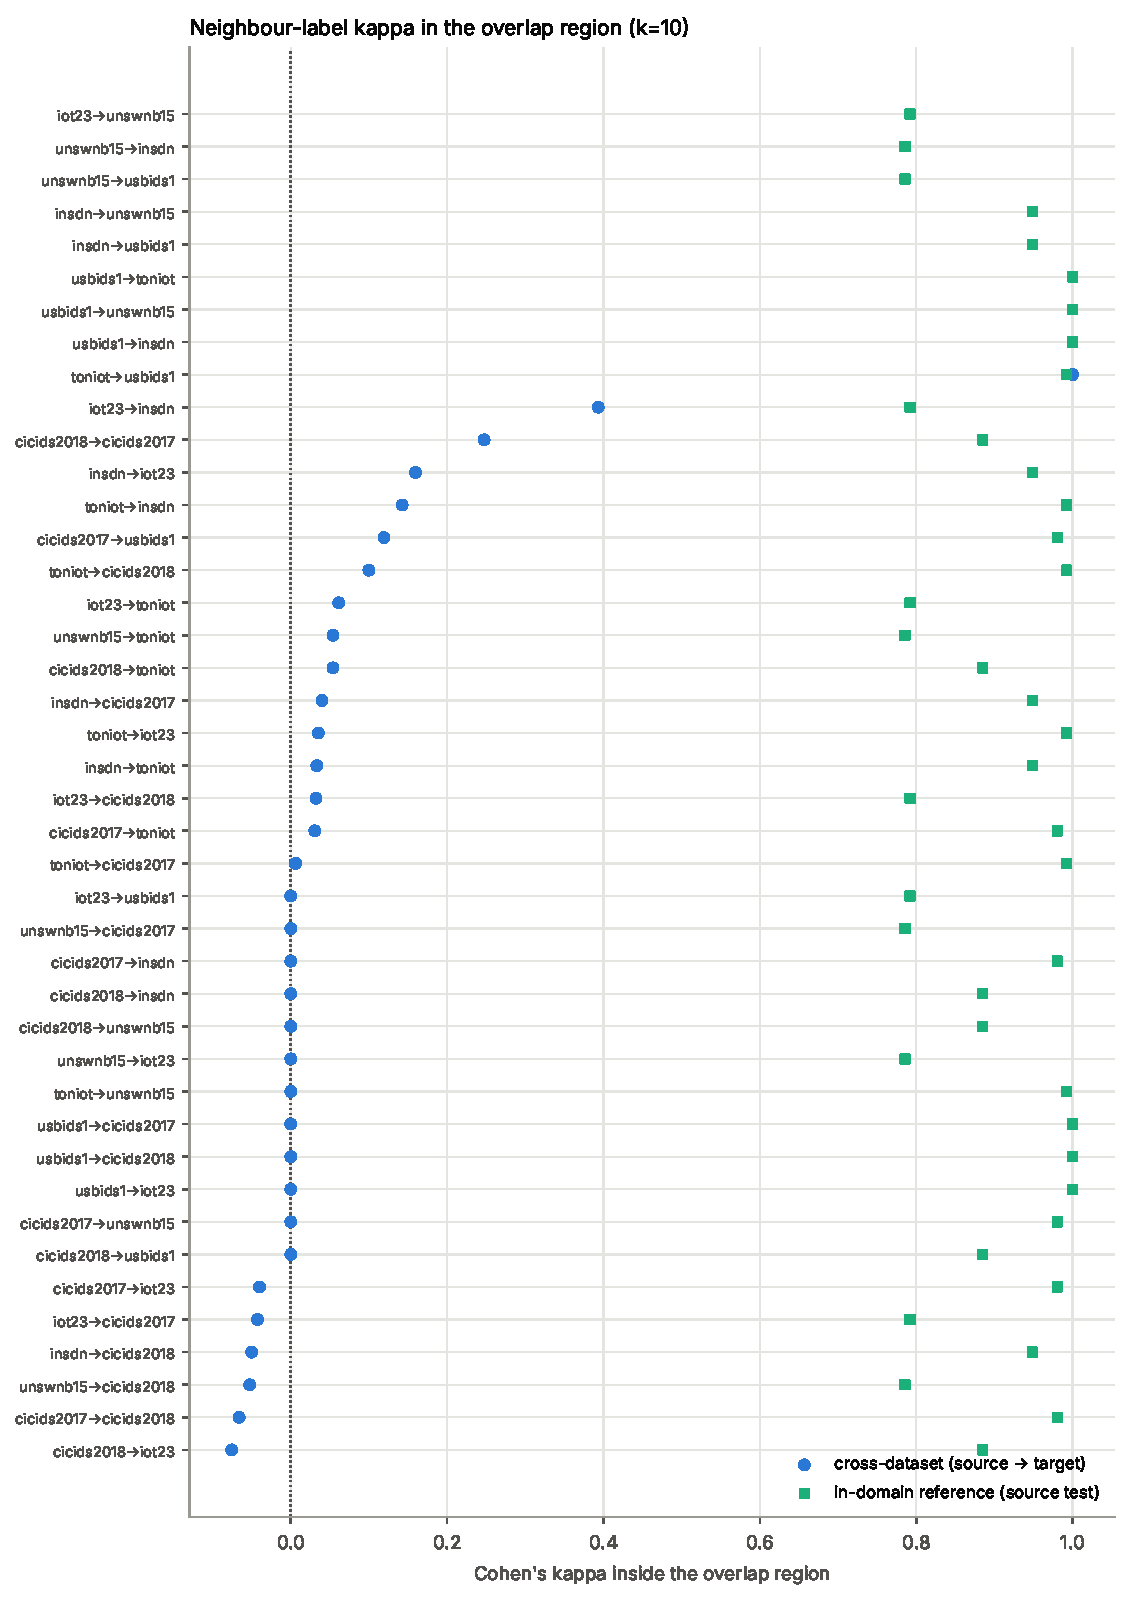
\includegraphics[width=0.8\textwidth]{figures/concept_kappa.pdf}
\caption{Cohen's $\kappa$ between the majority label of the nearest source rows and the true target label in the overlap region, per pair, against the in-domain reference.}\label{fig:kappa}
\end{figure}

\paragraph{No flow feature keeps its meaning.}
For each feature we computed the univariate ROC-AUC with the label in every dataset.
The sign of the association (above or below 0.5) is mixed for all 14 features of the eight datasets (13 core features and the minimal-tier \texttt{bytes\_per\_pkt}) and also for all 13 core features of the seven core datasets, with per-dataset AUC ranges such as 0.025 to 0.760 for total bytes and 0.057 to 0.808 for forward packets (Fig.~\ref{fig:sign}).

\begin{figure}[t]
\centering
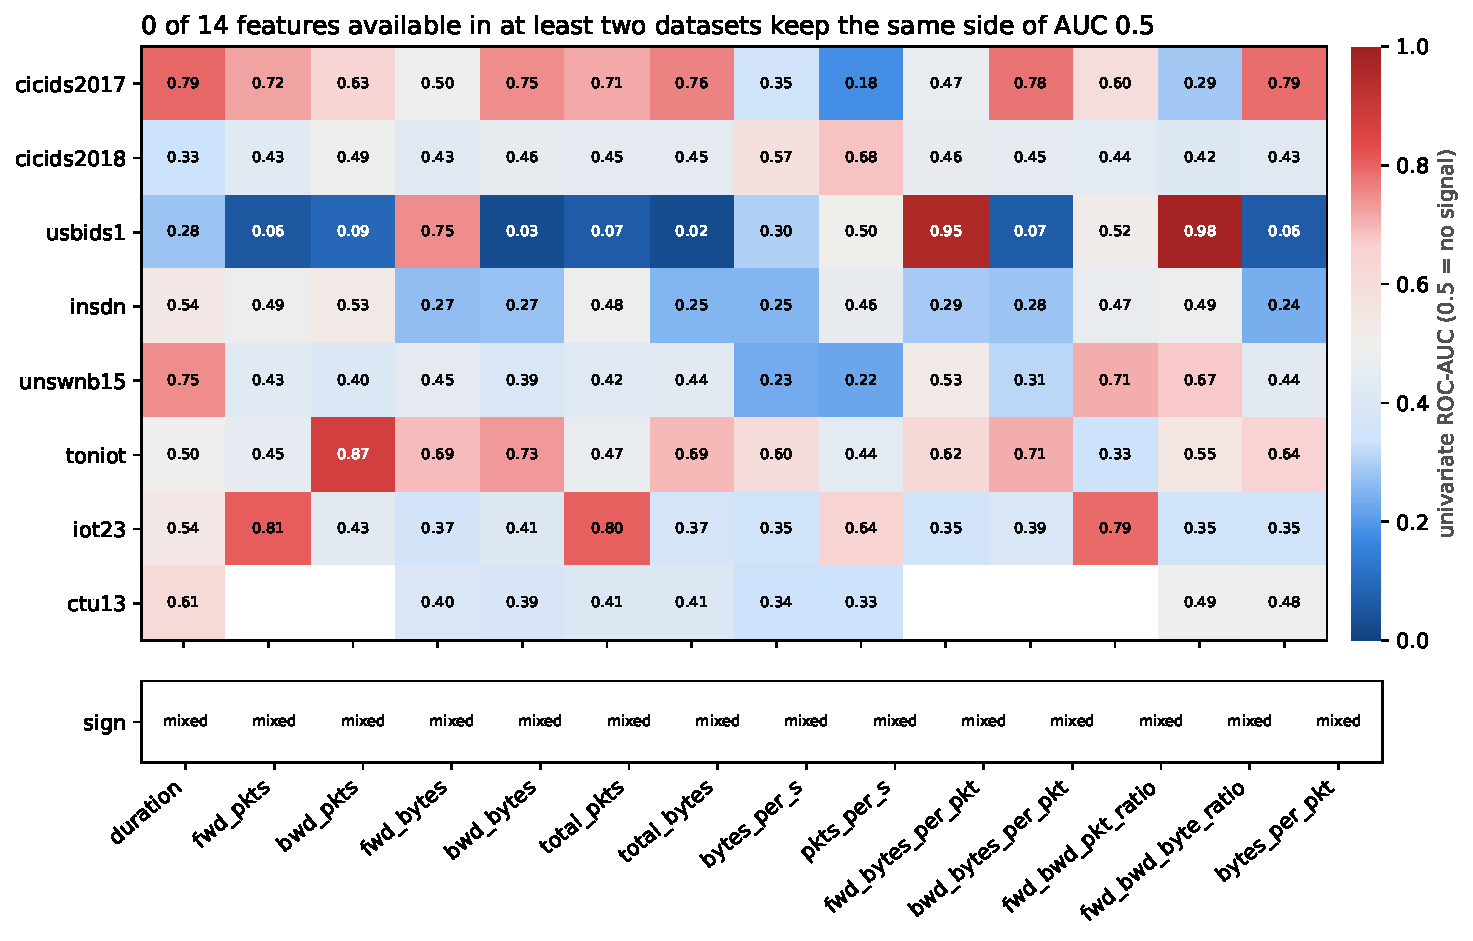
\includegraphics[width=0.9\textwidth]{figures/feature_sign.pdf}
\caption{Univariate ROC-AUC of each core feature with the attack label, per dataset (centred at 0.5); the figure includes CTU-13 and the minimal-tier feature \texttt{bytes\_per\_pkt}.}\label{fig:sign}
\end{figure}

\paragraph{Datasets are easy to tell apart.}
A CatBoost classifier recognises the dataset of a flow among the seven core datasets with 91.5\% accuracy (chance 14.3\%), and 91.8\% on benign flows alone.
Benign traffic therefore also differs between datasets, which is consistent with differences in capture setup and background traffic.

\paragraph{Published results agree.}
The reported collapses in the literature occur in the same regime: attack-class F1 below 1\% for several NetFlow-v2 pairs \citep{layeghy2023explainable}, MCC between 0.26 and 0.44 for CIC-IDS2017 and CIC-IDS2018 \citep{cantone2024crossdataset}.
Metrics and feature sets differ across studies, so we compare the pattern and not the numbers.

\section{Discussion}
The benchmark shows that cross-dataset transfer fails with every method we ran, and that the failure is not repaired by the usual remedies: tuning (on the pairs we tested), normalisation, feature selection, alignment, adversarial invariance, prior correction and self-training.
Below-chance ROC-AUC on 36 to 48\% of the pairs means that the source rule is not merely less informative on the target but inverted for a large share of the pairs, which a pure covariate shift would not produce.
The nearest-neighbour test, the per-feature sign flips and the failure of attack-family overlap to help all point the same way: the datasets disagree on which flows are labelled attacks.

\paragraph{What the evidence does not show.}
First, the evidence for a change in $P(y\mid x)$ is correlational.
Datasets differ in attack mix and benign background, and a per-feature sign flip arises when the attack mix differs, even without a labelling disagreement.
The nearest-neighbour test conditions on flow statistics but is restricted to the overlap region, which is small for most pairs (a median overlap fraction below 0.01), and a $\kappa$ near zero there means only that the neighbours' labels are uninformative, whichever way the shift is decomposed.
A per-attack-type comparison of the same attack in two laboratories, which would separate attack-mix shift from labelling disagreement, is not part of this study.
Second, the oracle control covers two pairs.
Third, the seven datasets are public laboratory captures with their own labelling errors \citep{engelen2021troubleshooting}, with only 13 harmonised flow features and no ports or payload, and the distinct-row sampling changes attack priors relative to natural traffic.
Fourth, RIFT is one design; the negative result concerns this design and these ablations.

\paragraph{Implications.}
Evaluation should report cross-dataset results with a pair taxonomy, because same-laboratory pairs can be the worst and one favourable pair hides the rest; a method that is not compared with its own baseline in the same setting, as here, can look useful for the wrong reason.
Methods that assume a fixed $P(y\mid x)$ should not be expected to repair these transfers, and the few-label results suggest that a few labelled flows of the target network are worth more than all the source data on average.

\section{Conclusion}
On eight public datasets, flow classifiers that reach 0.985 ROC-AUC in-domain reach 0.54 to 0.57 across datasets, with about 40\% of the transfers below chance, even between datasets from one laboratory.
A method designed for the covariate and label shifts of this setting (RIFT) is below its own baseline, and the failure is localised in the transductive components, above all in prior estimation.
Controls show that the datasets disagree on the labelling function and not only on scales, though the evidence is correlational and the oracle covers two pairs.
The practical consequence is that a handful of labelled flows from the target network is the reliable ingredient.

\paragraph{Reproducibility.}
The package, configurations, sampled-row hashes and every raw per-run result are in \url{https://github.com/vinhqdang/cross_ids}. Tables and figures are generated by \texttt{make\_benchmark\_tables.py} and \texttt{crossids analyze} from \texttt{results/runs.csv} and \texttt{results/controls}.

\bibliographystyle{plainnat}
\bibliography{refs}
\end{document}
